% **************************************************
% Document Class Definition
% **************************************************
\documentclass[%
	paper=A4,					% paper size --> A4 is default in Germany
	twoside=false,				% onesite or twoside printing
	%openright,					% doublepage cleaning ends up right side
	parskip=half,				% spacing value / method for paragraphs
	chapterprefix=true,			% prefix for chapter marks
	11pt,						% font size
	headings=normal,			% size of headings
	%bibliography=totoc,			% include bib in toc
	%listof=totoc,				% include listof entries in toc
	titlepageon,				% own page for each title page
	%captions=belowfigure,		% display table captions above the float env
	draft=false,				% value for draft version
]{scrreprt}%
\usepackage{ctex}
\usepackage{indentfirst}
\usepackage{booktabs}

% **************************************************
% Debug LaTeX Information
% **************************************************
%\listfiles

% **************************************************
% Information and Commands for Reuse
% **************************************************
\newcommand{\thesisSubTitle}{\heiti \bfseries 软件工程课程设计}
\newcommand{\thesisTitle}{\textsf{第二次报告}}

\newcommand{\thesisName}{\textit{\\[4.0cm] 
\textbf{姜华}\\[0.1cm]}}
\newcommand{\thesisSubject}{Documentation}
\newcommand{\thesisDate}{\today}
\newcommand{\thesisVersion}{2.1}


% **************************************************
% Load and Configure Packages
% **************************************************
\usepackage{listings}
\usepackage{color}
\usepackage[utf8]{inputenc}		% defines file's character encoding
\usepackage[english]{babel} % babel system, adjust the language of the content
\usepackage[					% clean thesis style
	figuresep=colon,%
	sansserif=false,%
	hangfigurecaption=false,%
	hangsection=true,%
	hangsubsection=true,%
	colorize=full,%
	colortheme=bluemagenta,%
	bibsys=bibtex,%
	bibfile=bib-refs,%
	bibstyle=alphabetic,%
]{cleanthesis}

\hypersetup{					% setup the hyperref-package options
	pdftitle={\thesisTitle},	% 	- title (PDF meta)
	pdfsubject={\thesisSubject},% 	- subject (PDF meta)
	pdfauthor={\thesisName},	% 	- author (PDF meta)
	plainpages=false,			% 	-
	colorlinks=false,			% 	- colorize links?
	pdfborder={0 0 0},			% 	-
	breaklinks=true,			% 	- allow line break inside links
	bookmarksnumbered=true,		%
	bookmarksopen=true			%
}
\definecolor{codegreen}{rgb}{0,0.6,0}
\definecolor{codegray}{rgb}{0.5,0.5,0.5}
\definecolor{codepurple}{rgb}{0.58,0,0.82}
\definecolor{backcolour}{rgb}{0.95,0.95,0.92}

\lstdefinestyle{mystyle}{
    backgroundcolor=\color{backcolour},   
    commentstyle=\color{codegreen},
    keywordstyle=\color{magenta},
    numberstyle=\tiny\color{codegray},
    stringstyle=\color{codepurple},
    basicstyle=\footnotesize,
    breakatwhitespace=false,         
    breaklines=true,                 
    captionpos=b,                    
    keepspaces=true,                 
    numbers=left,                    
    numbersep=5pt,                  
    showspaces=false,                
    showstringspaces=false,
    showtabs=false,                  
    tabsize=2
}



\lstdefinestyle{styleJ}{
    language=Java,
    keywordstyle=\color{keywordcolor}\bfseries, 
    commentstyle=\color{blue} \textit, 
    showstringspaces=false,
    numbers=left,
    numberstyle=\small
}
\lstset{style=styleJ}



\usepackage{xcolor}
\usepackage{listings}
\usepackage{fontspec}
\usepackage{tikz}
\usepackage{wrapfig}
\usepackage{floatrow}
\usepackage{multirow}
\usepackage[justification=centering]{caption}
\usepackage{longtable}
\usepackage{float}
%\newfontfamily\menlo{Menlo} %Menlo
%\newfontfamily\cons{Consolas}
%\newfontfamily\moki{mononoki}
\lstset{
    %numbers=left,
    tabsize=4,
    numberstyle= \footnotesize, 
    %frame=shadowbox, % 阴影效果
    rulesepcolor= \color{ red!20!green!20!blue!20} ,
    escapeinside=``, % 英文分号中可写入中文
    xleftmargin=2em,xrightmargin=0em, aboveskip=1em,
    framexleftmargin=2em,    
    columns=fixed,         
    %numbers=left,                                        % 在左侧显示行号  
    frame=none,                                          % 不显示背景边框  
    %backgroundcolor=\color[RGB]{240,240,240},            % 设定背景颜色  
    keywordstyle=\bfseries\color[RGB]{60,60,220},                 % 设定关键字颜色  
    numberstyle=\footnotesize\color{darkgray},           % 设定行号格式  
    commentstyle=\it\color[RGB]{0,96,96},                % 设置代码注释的格式  
    stringstyle=\rmfamily\slshape\color[RGB]{128,0,0},   % 设置字符串格式  
    showstringspaces=false,                              % 不显示字符串中的空格    
    otherkeywords={string, Type, NULL},
    basicstyle=\footnotesize\cons ,
}
\usepackage{caption}

\DeclareCaptionFont{white}{ \color{black} }
\DeclareCaptionFormat{listing}{
	\centering #1#2#3
%  \colorbox[cmyk]{0.43, 0.35, 0.35,0.01 }{
%    \parbox{\textwidth}{\hspace{15pt}#1#2#3}
%  }
}
\captionsetup[lstlisting]{ format=listing, labelfont=white, textfont=white, singlelinecheck=false, margin=0, font={bf,small} }

% ...

%\lstinputlisting[caption=My caption]{sourcefile.lang}

\geometry{a4paper,scale=0.99}

% **************************************************
% Document CONTENT
% **************************************************
\begin{document}

% --------------------------
% rename document parts
% --------------------------
%\renewcaptionname{ngerman}{\figurename}{Abb.}
%\renewcaptionname{ngerman}{\tablename}{Tab.}
\renewcaptionname{english}{\figurename}{Fig}
\renewcaptionname{english}{\tablename}{Tab.}
\renewcommand\contentsname{Contents}
% \renewcommand\listtablename{Table Index}
\renewcommand\listfigurename{Image Index}


% --------------------------
% Front matter
% --------------------------
\pagenumbering{roman}			% roman page numbing (invisible for empty page style)
\pagestyle{empty}				% no header or footers
% !TEX root = ../thesis.tex
%
% ------------------------------------  --> cover title page
\newgeometry{top=2.5cm,bottom=2cm,left=2cm,right=2cm}
\begin{titlepage}
	\pdfbookmark[0]{Cover}{Cover}
	\begin{minipage}{0.2\textwidth}
	
\includegraphics[width=\textwidth]{./gfx/tj.jpg}
	\end{minipage}
	\begin{minipage}{0.7\textwidth}
	\flushright
		\textit{\color{ctcolortitle}\thesisDate} \\
		{\color{ctcolortitle}Edition: \thesisVersion }
	\end{minipage}
	%\flushright
	\centering
		\\[4cm]
	{\Large \thesisSubTitle }\\
	{\color{ctcolortitle}\rule[1pt]{0.9\textwidth}{.4pt}} \\
	{\Huge\color{ctcolortitle}\thesisTitle \\}
	\vspace{0.3cm}
	{\color{ctcolortitle}\rule[3pt]{0.9\textwidth}{.4pt}} \\
	{\large\thesisName}
	\vfill
	{\kaishu{\Large  {软件工程课程设计}}\\[0.1cm]
	\color{ctcolortitle}\kaishu{\large Tongji University}\\
	\textsc{\large  School of Software Engineering}\\[0.5cm]}
	%
\includegraphics[width=0.4\textwidth]{./gfx/tj.jpg}

\end{titlepage}


% ------------------------------------  --> main title page
%\begin{titlepage}
%	\pdfbookmark[0]{Titlepage}{Titlepage}
%	\tgherosfont
%	\centering
%
%	{\Large \thesisUniversity} \\[4mm]
%	\includegraphics[width=6cm]{gfx/Clean-Thesis-Logo} \\[2mm]
%	\textsf{\thesisUniversityDepartment} \\
%	\textsf{\thesisUniversityInstitute} \\
%	\textsf{\thesisUniversityGroup} \\
%
%	\vfill
%	{\large \thesisSubject} \\[5mm]
%	{\LARGE \color{ctcolortitle}\textbf{\thesisTitle} \\[10mm]}
%	{\Large \thesisName} \\
%
%	\vfill
%	\begin{minipage}[t]{.27\textwidth}
%		\raggedleft
%		\textit{1. Reviewer}
%	\end{minipage}
%	\hspace*{15pt}
%	\begin{minipage}[t]{.65\textwidth}
%		{\Large \thesisFirstReviewer} \\
%	  	{\small \thesisFirstReviewerDepartment} \\[-1mm]
%		{\small \thesisFirstReviewerUniversity}
%	\end{minipage} \\[5mm]
%	\begin{minipage}[t]{.27\textwidth}
%		\raggedleft
%		\textit{2. Reviewer}
%	\end{minipage}
%	\hspace*{15pt}
%	\begin{minipage}[t]{.65\textwidth}
%		{\Large \thesisSecondReviewer} \\
%	  	{\small \thesisSecondReviewerDepartment} \\[-1mm]
%		{\small \thesisSecondReviewerUniversity}
%	\end{minipage} \\[10mm]
%	\begin{minipage}[t]{.27\textwidth}
%		\raggedleft
%		\textit{Supervisors}
%	\end{minipage}
%	\hspace*{15pt}
%	\begin{minipage}[t]{.65\textwidth}
%		\thesisFirstSupervisor\ and \thesisSecondSupervisor
%	\end{minipage} \\[10mm]
%
%	\thesisDate \\
%
%\end{titlepage}
%
%
%% ------------------------------------  --> lower title back for single page layout
%\hfill
%\vfill
%{
%	\small
%	\textbf{\thesisName} \\
%	\textit{\thesisTitle} \\
%	\thesisSubject, \thesisDate \\
%	Reviewers: \thesisFirstReviewer\ and \thesisSecondReviewer \\
%	Supervisors: \thesisFirstSupervisor\ and \thesisSecondSupervisor \\[1.5em]
%	\textbf{\thesisUniversity} \\
%	\textit{\thesisUniversityGroup} \\
%	\thesisUniversityInstitute \\
%	\thesisUniversityDepartment \\
%	\thesisUniversityStreetAddress \\
%	\thesisUniversityPostalCode\ and \thesisUniversityCity
%}
\restoregeometry		% INCLUDE: all titlepages
%\cleardoublepage

%\pagestyle{plain}				% display just page numbers
%\input{content/abstract}		% INCLUDE: the abstracts (english and german)
%\cleardoublepage
%
%\input{content/acknowledgement} % INCLUDE: acknowledgement
%\cleardoublepage
%
\newgeometry{top=1cm,bottom=1cm}
\setcounter{tocdepth}{2}		% define depth of toc
\tableofcontents				% display table of contents
\restoregeometry
%\cleardoublepage

% --------------------------
% Body matter
% --------------------------
\pagenumbering{arabic}			% arabic page numbering
\setcounter{page}{2}			% set page counter
\pagestyle{maincontentstyle} 	% fancy header and footer

\chapter{Part 1\  循环神经网络}

\section{RNN}
\text{用于处理序列,处理序列(例如文本)的方式是,遍历序列中的所有元素,并保存一个状态,其中包含已查看内容的相关信息。}





\begin{figure}[H]
	\centering
	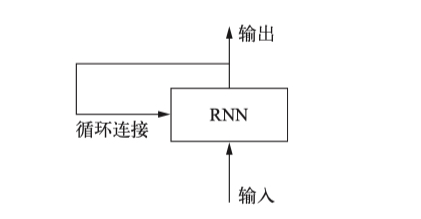
\includegraphics[width = 1.2\columnwidth]{InmemoryDatabaseExperiment/fig/2rnn1.jpg}
	\caption{RNN}
\end{figure}

\text{在处理两个不同的独立序列之间,RNN的状态都会被重置。所以仍然可以将一个序列看作单个数据点,即网络的输入。真正改变的是,数据点不再是在单个步骤中进行处理, 相反,网络内部会对序列元素进行遍历。}
\subsection{RNN的前向传递过程}

\begin{figure}[H]
	\centering
	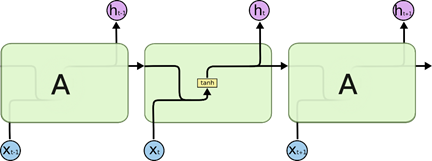
\includegraphics[width = 1.2\columnwidth]{InmemoryDatabaseExperiment/fig/rnn3.png}
	\caption{RNN前向传播}
\end{figure}
\text{如图是三个神经网络,上一个网络的信息(即ht-1)直接传过来,配合当前网络的输入Xt,两者结合之后,再通过tanh层进行信息压缩,就形成当前网络的输出ht。(这个tanh层就是一个函数,tanh就是双曲正切函数,可以将输入的值转化为-1到1之间的一个值,通常用于对信息的压缩处理,或者规范化处理。)}


\section{LSTM (长短期记忆网络)}

\text{LSTM 层是 SimpleRNN 层的一种变体,它增加了一种携带信息跨越多个时间步的方法。}
\begin{figure}[H]
	\centering
	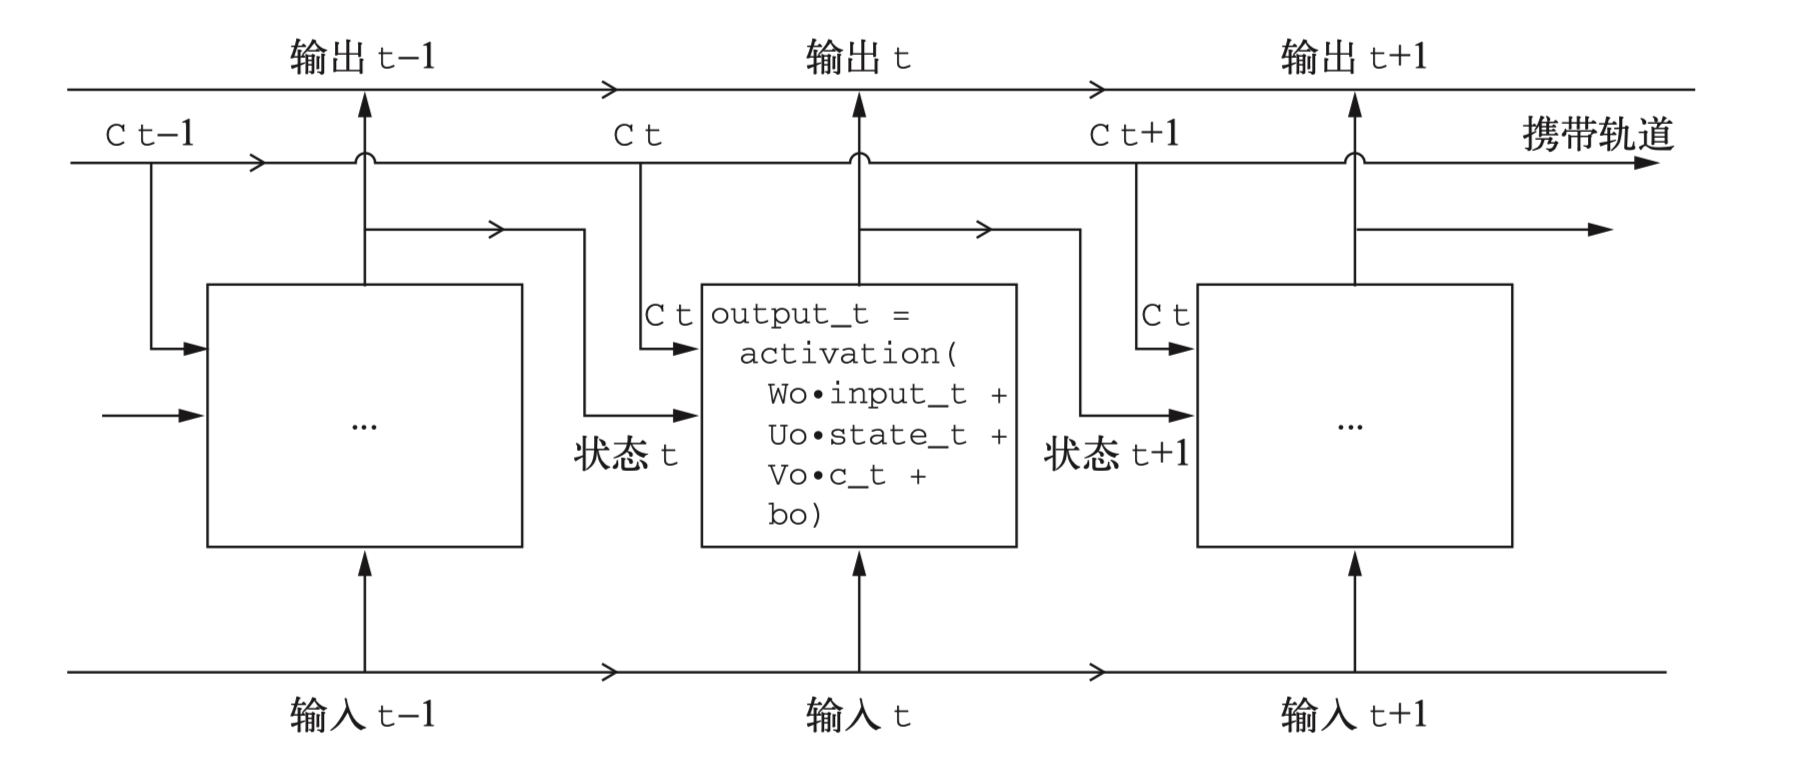
\includegraphics[width = 1.2\columnwidth]{InmemoryDatabaseExperiment/fig/lstm_2.jpg}
	\caption{LSTM}
\end{figure}

\text{我们向这张图像中添加额外的数据流,其中携带着跨越时间步的信息。它在不同的时间步 的值叫作 Ct ,其中 C 表示携带(carry)。Ct的计算方法和当前状态有关,从而会影响传递到下一个时间步的状态。}

\section{C-LSTM for text classification}


\begin{figure}[H]
	\centering
	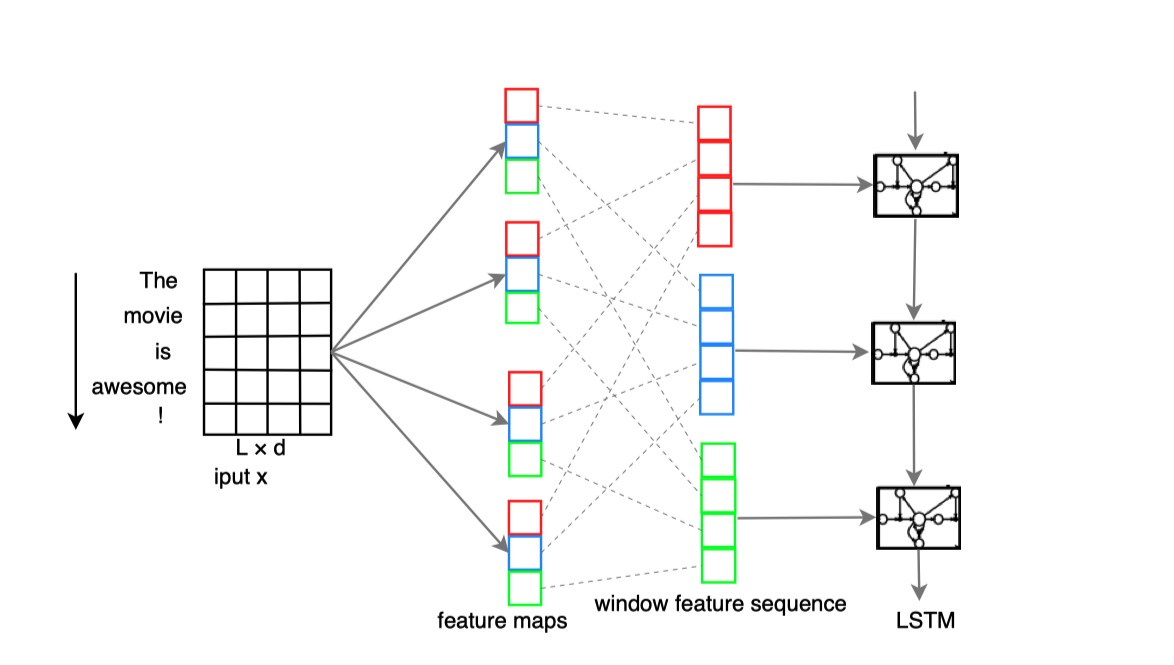
\includegraphics[width = 1.2\columnwidth]{InmemoryDatabaseExperiment/fig/clstm_2.jpg}
	\caption{C-LSTM}
\end{figure}

\subsection{一维卷积神经网络}
\text{图中的一维卷积神经网络有四个filter,每一个filter都有一个宽度为k的窗口向量,用这个窗口向量对文本序列进行划窗,本图中是划窗3次,生成一个特征图(feature map),用三种不同的颜色来代表一个filter的不同划窗的计算结果,红色,蓝色,绿色的方块代表的计算结果具有位置上的先后关系。}
\text{把所有filter的计算结果按照划窗顺序聚集在一起(相同颜色的方块放在一起),然后输入给LSTM}
\text{在LSTM的最后一步的输出后加上一softmax层,然后进行训练。}





\chapter{Part 2\  Experiment}

\section{目标}
\text{文本分类}
\section{模型}
\text{C-LSTM}
\section{数据格式(训练数据和测试数据)}
数据存储在csv文件中,分为两列,“label”列和“content”列,分别代表一条文本序列的类别和内容,总共有两类

\begin{figure}[H]
	\centering
	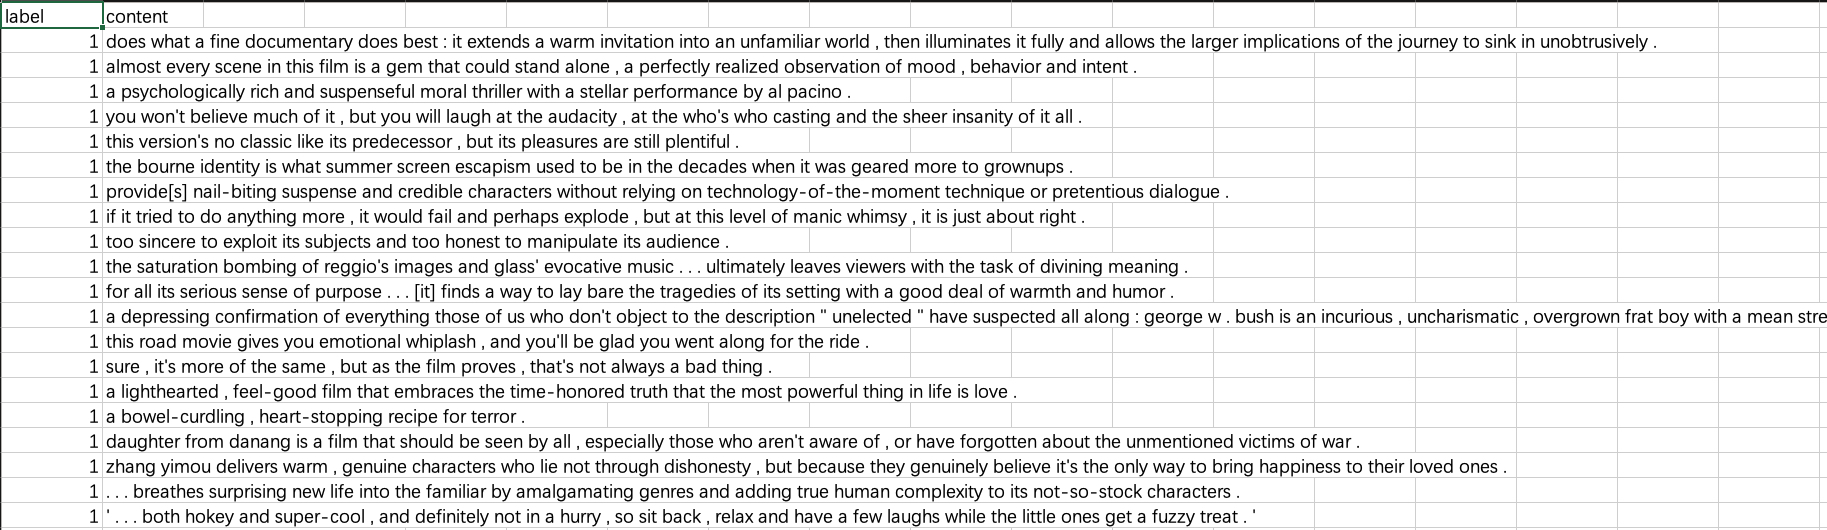
\includegraphics[width = 1.2\columnwidth]{InmemoryDatabaseExperiment/fig/data1.jpg}
	\caption{C-LSTM}
\end{figure}

\section{训练以及验证}
\begin{itemize}
    \item 使用4500条“label1”的文本和4500条“label2”的文本进行训练
    \item 在450条“label1”的文本和450条“label2”的文本上进行验证
\end{itemize}

\section{Result}

\text{在作为验证集的1000条文本中获得了76.6\%的准确率}
\begin{figure}[H]
	\centering
	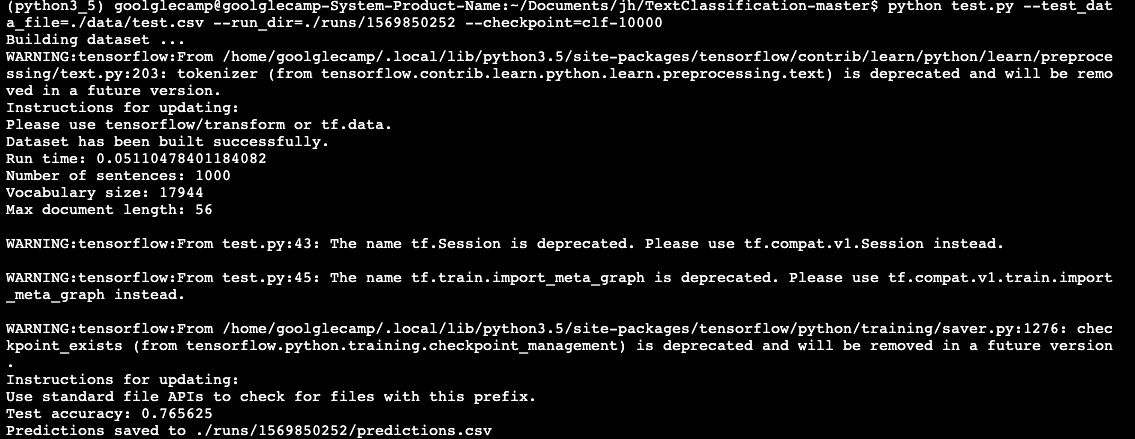
\includegraphics[width = 1.2\columnwidth]{InmemoryDatabaseExperiment/fig/predict.jpg}
	\caption{验证结果}
\end{figure}


\chapter{Part 3\  下一步工作}
\begin{itemize}
    \item 学习使用C-LSTM对异常数据序列进行分类
\end{itemize}



\chapter{Appendix A}
\listoffigures

% \chapter{Appendix B}
% \listoftables





% --------------------------
% Back matter
% --------------------------
{%
\setstretch{1.1}
\renewcommand{\bibfont}{\normalfont\small}
\setlength{\biblabelsep}{0pt}
\setlength{\bibitemsep}{0.5\baselineskip plus 0.5\baselineskip}
\printbibliography[nottype=online]
\printbibliography[heading=subbibliography,title={Webseiten},type=online,prefixnumbers={@}]
}
%\cleardoublepage
%
%\listoffigures
%\cleardoublepage
%
%\listoftables
%\cleardoublepage
%
%%\input{content/colophon}
%%\cleardoublepage
%
%%\input{content/declaration}
%\clearpage
%\newpage
%\mbox{}

% **************************************************
% End of Document CONTENT
% **************************************************
\end{document}
